\subsection{Эмпирическая функция распределения}

\begin{figure}[H]
	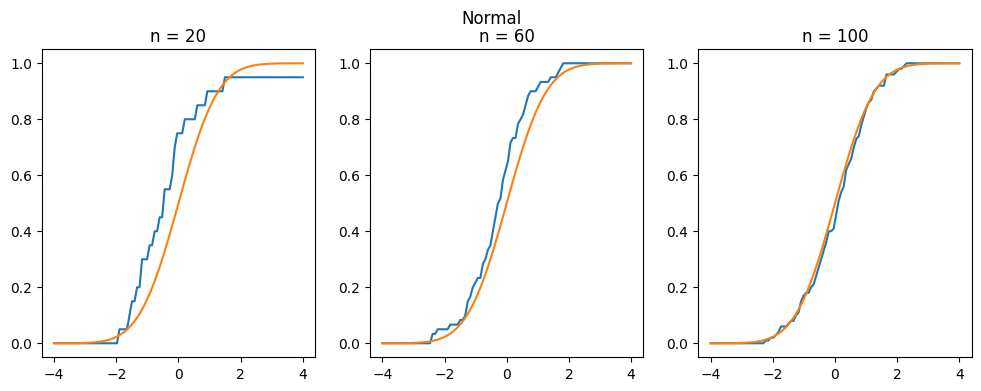
\includegraphics[width=\textwidth]{tasks/4/res/1.png}
	\caption{Нормальное распределение} 
\end{figure}
	
\begin{figure}[H]
	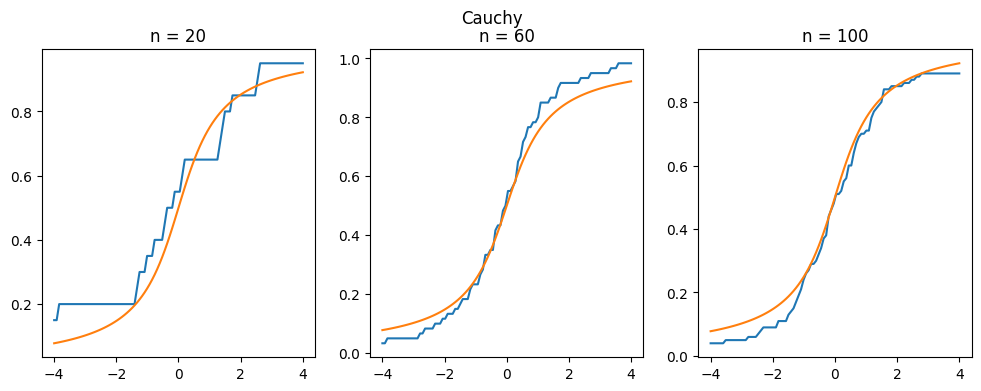
\includegraphics[width=\textwidth]{tasks/4/res/2.png}
	\caption{Распределение Коши} 
\end{figure}
	
\begin{figure}[H]
	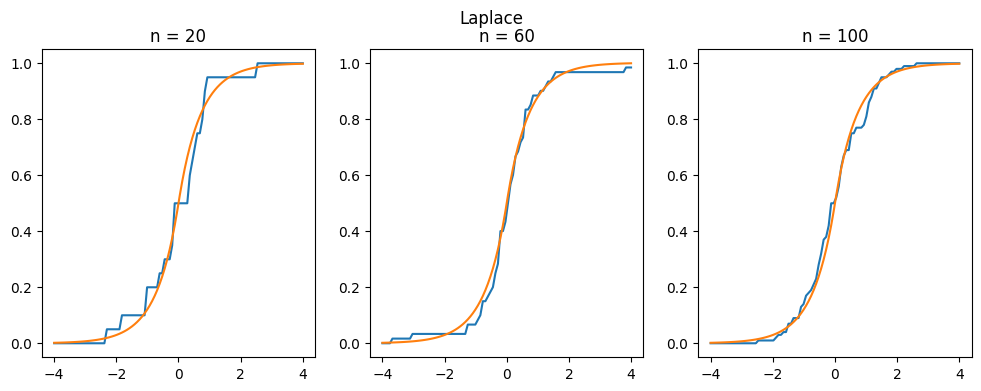
\includegraphics[width=\textwidth]{tasks/4/res/3.png}
	\caption{Распределение Лапласа} 
\end{figure}
	
\begin{figure}[H]
	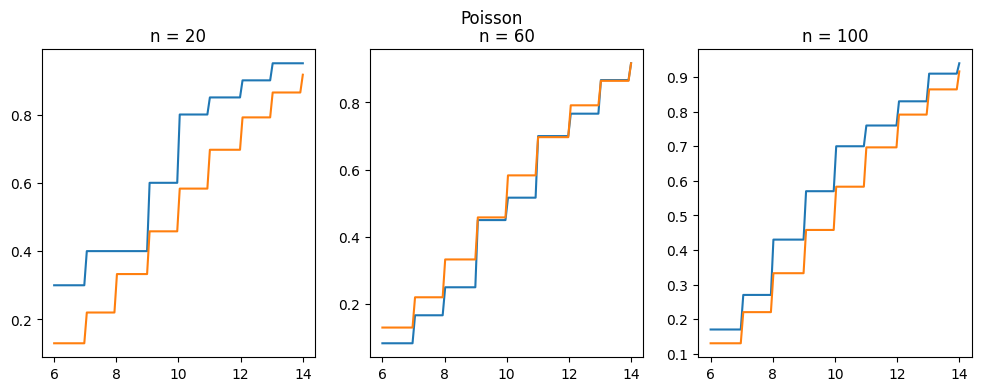
\includegraphics[width=\textwidth]{tasks/4/res/4.png}
	\caption{Распределение Пуассона} 
\end{figure}
	
\begin{figure}[H]
	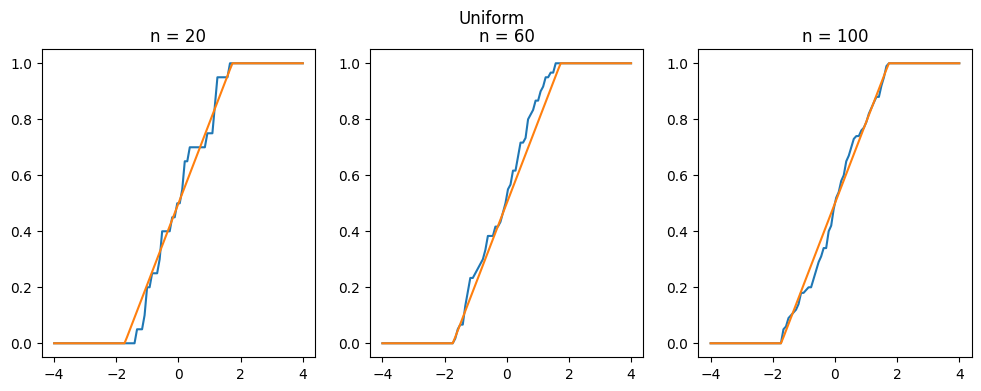
\includegraphics[width=\textwidth]{tasks/4/res/5.png}
	\caption{Равномерное распределение} 
\end{figure}
	
\subsection{Ядерные оценки плотности распределения}
\begin{figure}[H]
	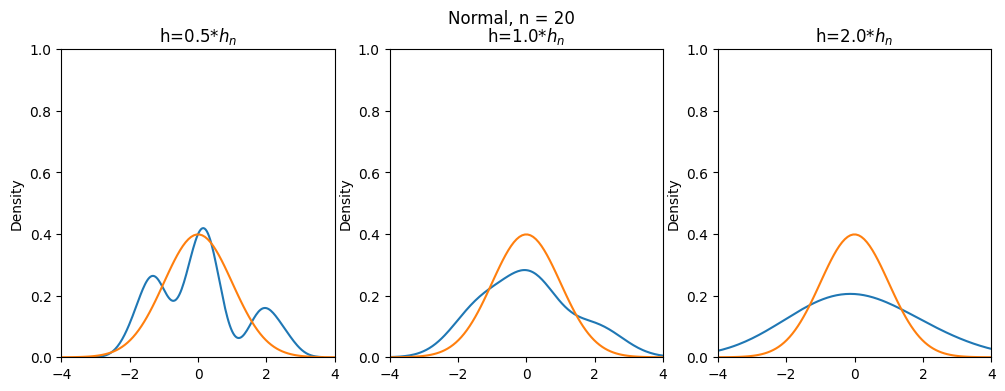
\includegraphics[width=\textwidth]{tasks/4/res/11.png}
	\caption{Нормальное распределение, n = 20} 
\end{figure}
	
\begin{figure}[H]
	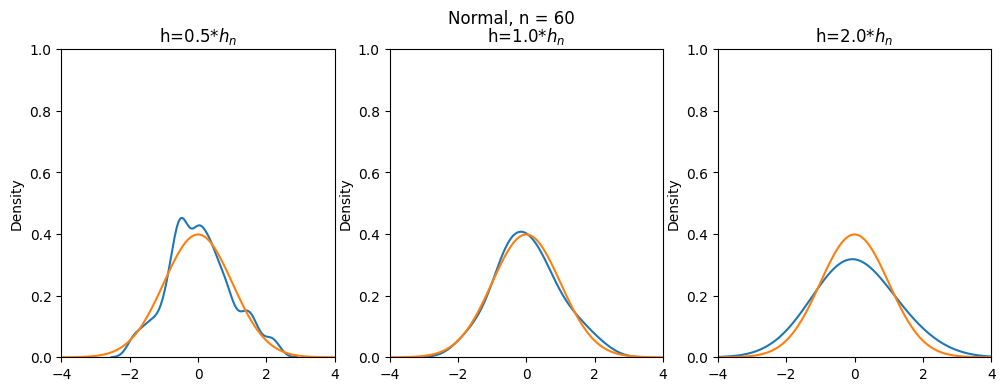
\includegraphics[width=\textwidth]{tasks/4/res/12.png}
	\caption{Нормальное распределение, n = 60} 
\end{figure}
	
\begin{figure}[H]
	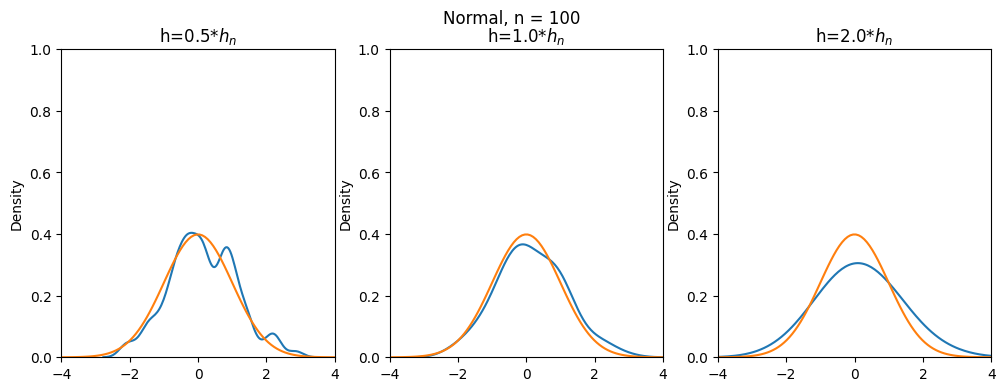
\includegraphics[width=\textwidth]{tasks/4/res/13.png}
	\caption{Нормальное распределение, n = 100} 
\end{figure}
	
\begin{figure}[H]
	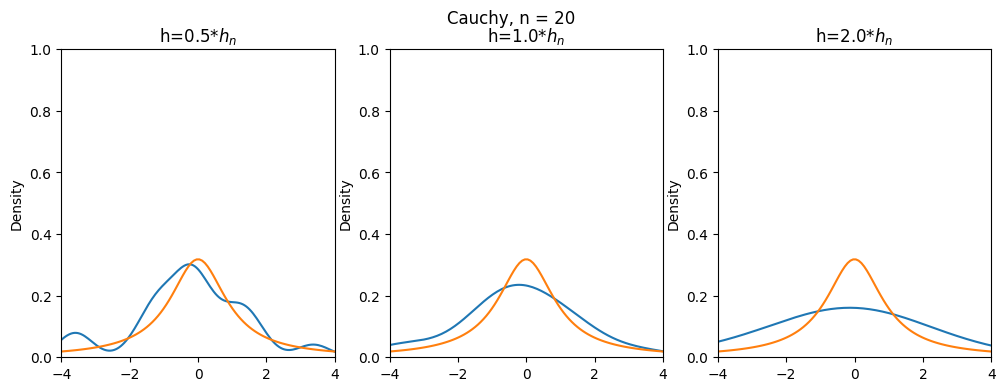
\includegraphics[width=\textwidth]{tasks/4/res/21.png}
	\caption{Распределение Коши, n = 20} 
\end{figure}
	
\begin{figure}[H]
	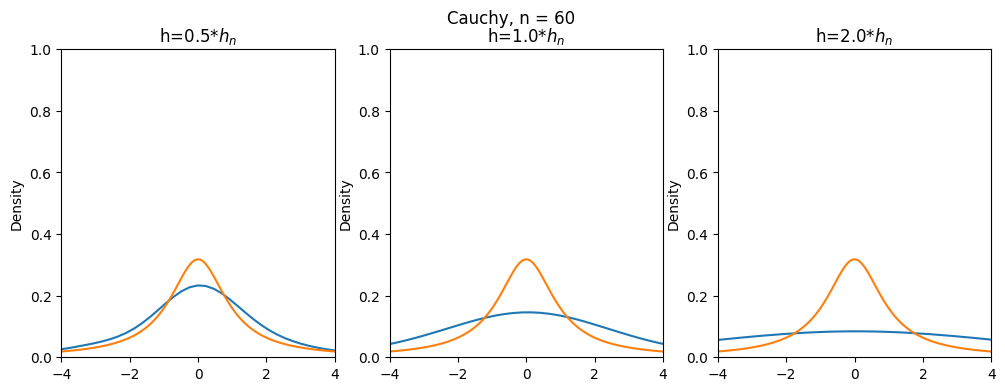
\includegraphics[width=\textwidth]{tasks/4/res/22.png}
	\caption{Распределение Коши, n = 60} 
\end{figure}
	
\begin{figure}[H]
	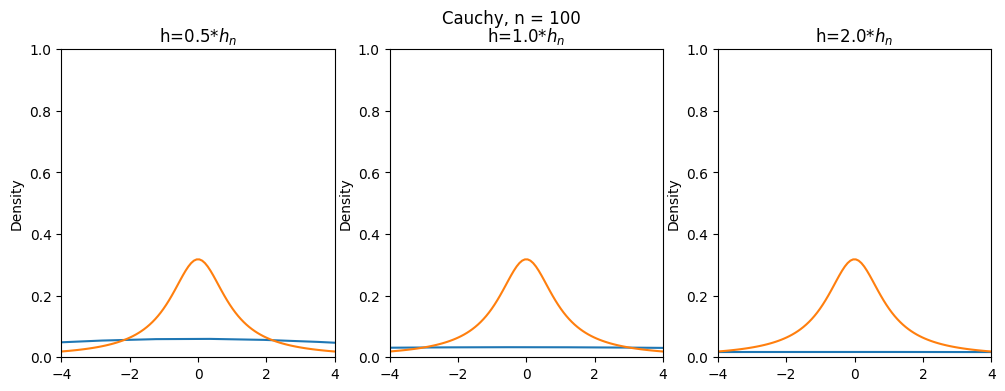
\includegraphics[width=\textwidth]{tasks/4/res/23.png}
	\caption{Распределение Коши, n = 100} 
\end{figure}
	
\begin{figure}[H]
	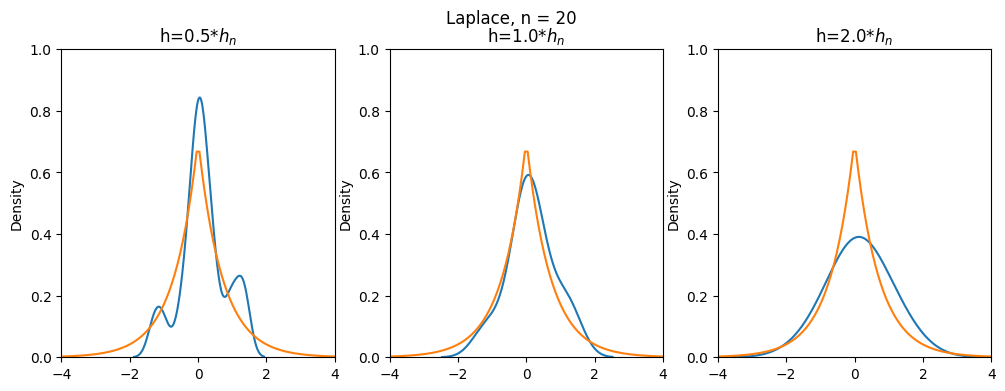
\includegraphics[width=\textwidth]{tasks/4/res/31.png}
	\caption{Распределение Лапласа, n = 20} 
\end{figure}
	
\begin{figure}[H]
	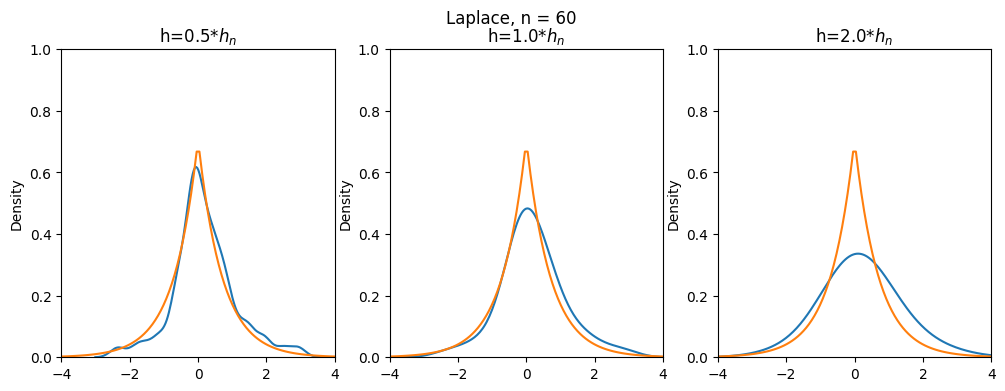
\includegraphics[width=\textwidth]{tasks/4/res/32.png}
	\caption{Распределение Лапласа, n = 60} 
\end{figure}
	
\begin{figure}[H]
	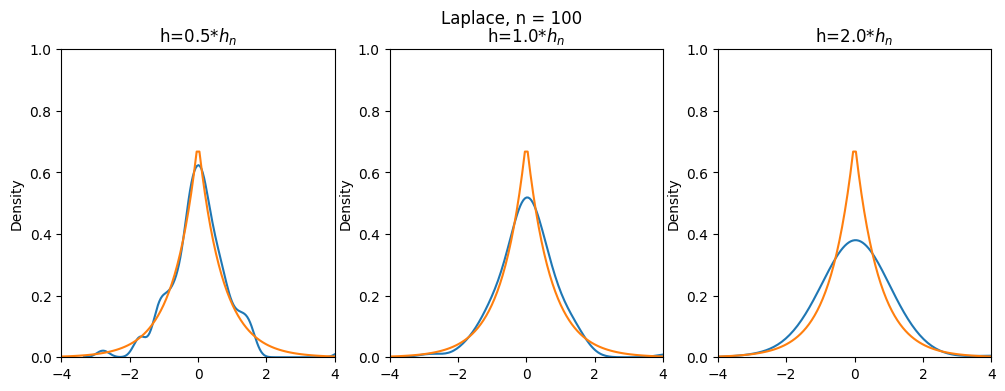
\includegraphics[width=\textwidth]{tasks/4/res/33.png}
	\caption{Распределение Лапласа, n = 100} 
\end{figure}
	
\begin{figure}[H]
	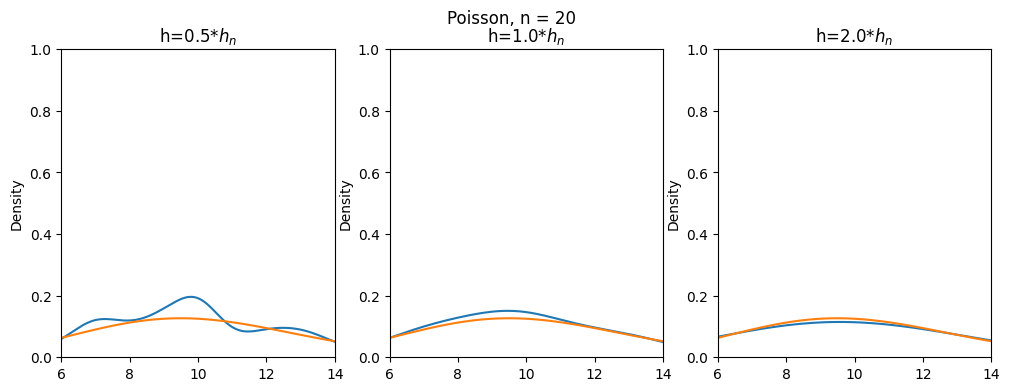
\includegraphics[width=\textwidth]{tasks/4/res/41.png}
	\caption{Распределение Пуассона, n = 20} 
\end{figure}
	
\begin{figure}[H]
	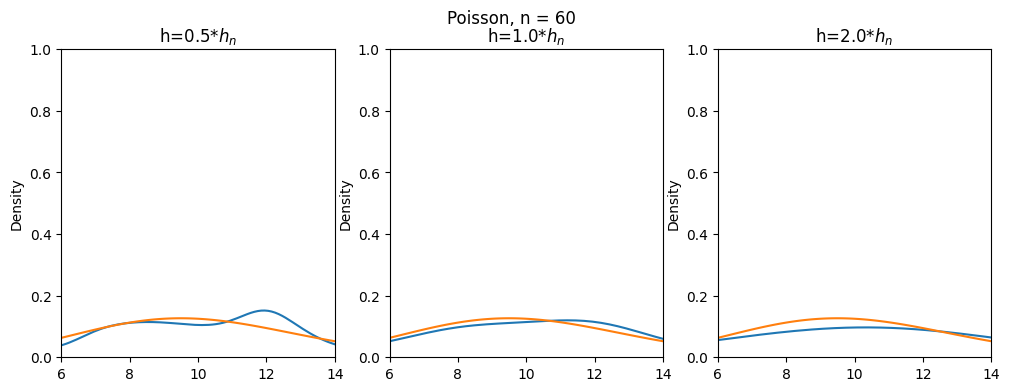
\includegraphics[width=\textwidth]{tasks/4/res/42.png}
	\caption{Распределение Пуассона, n = 60} 
\end{figure}
	
\begin{figure}[H]
	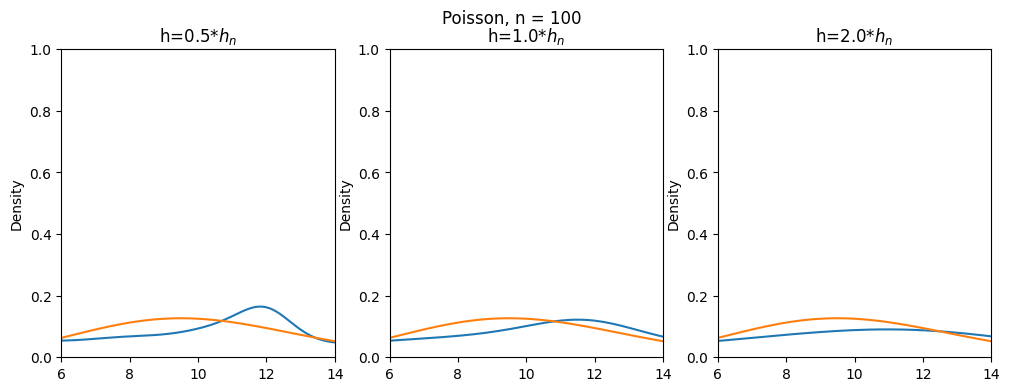
\includegraphics[width=\textwidth]{tasks/4/res/43.png}
	\caption{Распределение Пуассона, n = 100} 
\end{figure}
	
\begin{figure}[H]
	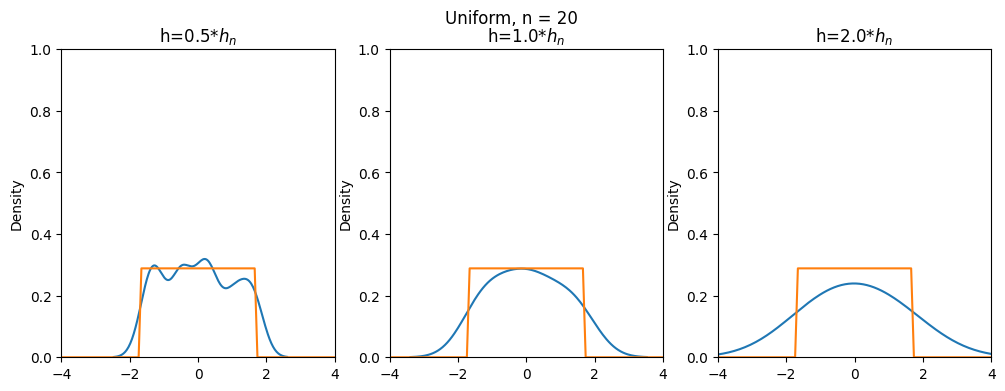
\includegraphics[width=\textwidth]{tasks/4/res/51.png}
	\caption{Равномерное распределение, n = 20} 
\end{figure}

\begin{figure}[H]
	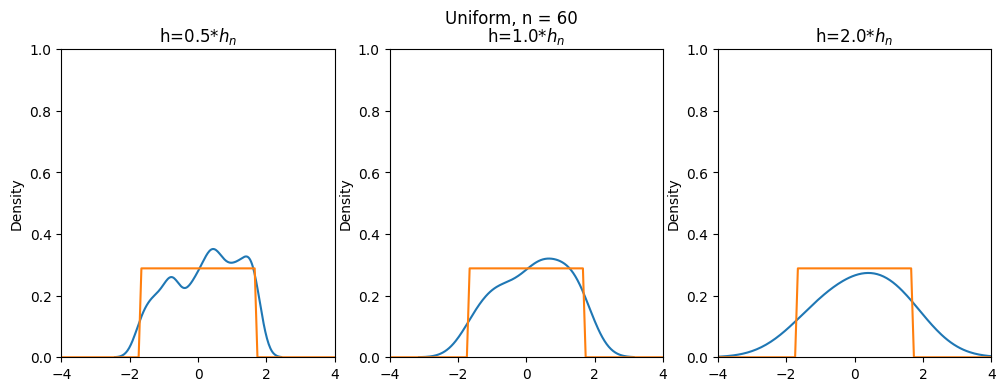
\includegraphics[width=\textwidth]{tasks/4/res/52.png}
	\caption{Равномерное распределение, n = 60} 
\end{figure}

\begin{figure}[H]
	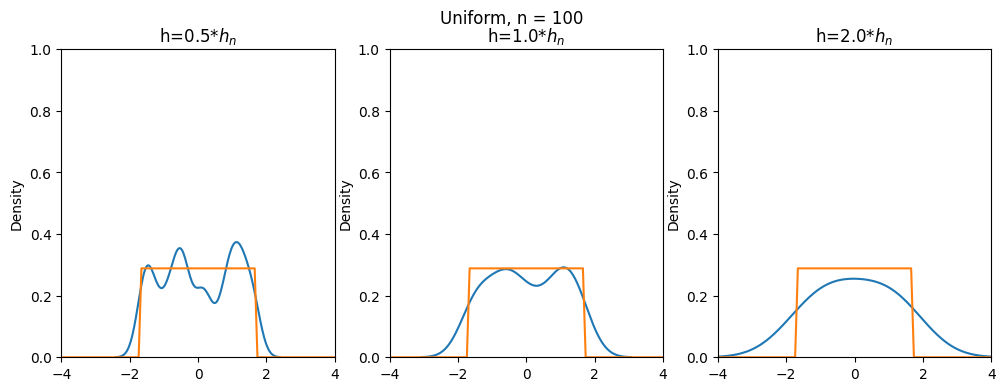
\includegraphics[width=\textwidth]{tasks/4/res/53.png}
	\caption{Равномерное распределение, n = 100} 
\end{figure}
